\section{Aprendizaje profundo}

\subsection{Redes neuronales}

Una red neuronal se llama así porque los científicos intentaron modelar el cerebro en código informático. El objetivo final es crear una “inteligencia general artificial”, en otras palabras un programa que puede aprender todo lo que una persona podria aprender.

Las redes neuronales artificiales son una clase de algoritmos de aprendizaje máquina que aprenden de los datos y se especializan en el reconocimiento de patrones (\cite{rosebrock2017deep}).

Una red neuronal es una función flexible que adapta de manera autónoma su comportamiento para satisfacer la relación entre la entradas y los resultados esperados y se ha denominado como un aproximador universal (\cite{goyal2018Deep}).

\subsection{Perceptrón}

Rosenblatt publicó el algoritmo seminal Perceptron: este modelo podía aprender automáticamente los pesos necesarios para clasificar una entrada.

Perceptron toma n entradas y produce una única salida binaria si la suma es mayor que el valor de activación. Se dice que la neurona se "dispara" siempre que se excede el valor de activación y se comporta como una función escalonada, lo cual se muestra en la ecuación \ref{eq:fnStep} (\cite{goyal2018Deep}).

\begin{equation}
\label{eq:fnStep}
    f\left(x\right)=\begin{cases}0 & x -u < 0\\1 & x -u >= 0\end{cases}
\end{equation}



Minsky y Papert demostraron que un perceptrón con una función de activación lineal es simplemente un clasificador lineal, incapaz de resolver problemas no lineales (\cite{rosebrock2017deep}). El ejemplo canónico de un problema no lineal es el conjunto de datos XOR Figura \ref{fig:xor}.

Perceptron se puede convertir fácilmente en un algoritmo en línea que procesa un flujo de ejemplos, actualizando el vector de peso solo si el último ejemplo recibido está mal clasificado. Se garantiza que el perceptrón convergerá en una solución si los datos de entrenamiento son linealmente separables, pero de lo contrario no convergerán(\cite{flach2012Machine}).

\begin{figure}[H]
    \centering
    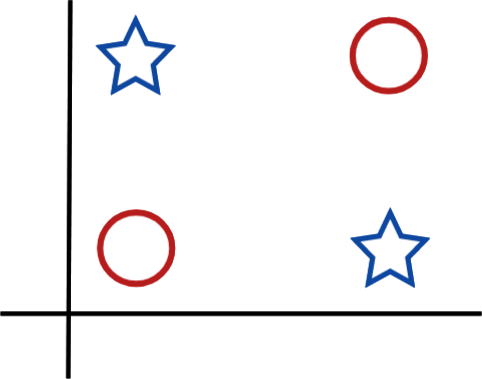
\includegraphics[width=0.5\textwidth]{MarcoTeorico/imgs/XOR.png}
    \caption{Problema XOR, no es linealmente separable.}
    \label{fig:xor}
\end{figure}


\subsection{Redes Neuronales Multicapa}


Los perceptrones multicapa o MLP (Multilayer Perceptron) son una red neuronal de propagación hacia adelante y se componen de múltiples perceptrones conectados entre sí y que operan en funciones de activación distintivas para permitir mejores mecanismos de aprendizaje. La arquitectura perceptrón multicapa cuenta como mínimo con 3 capas: una capa de entrada, una o más capas ocultas y una capa de salida (\cite{swamynathan2017Mastering}) Figura \ref{fig:mlp}.

\begin{figure}[H]
    \centering
    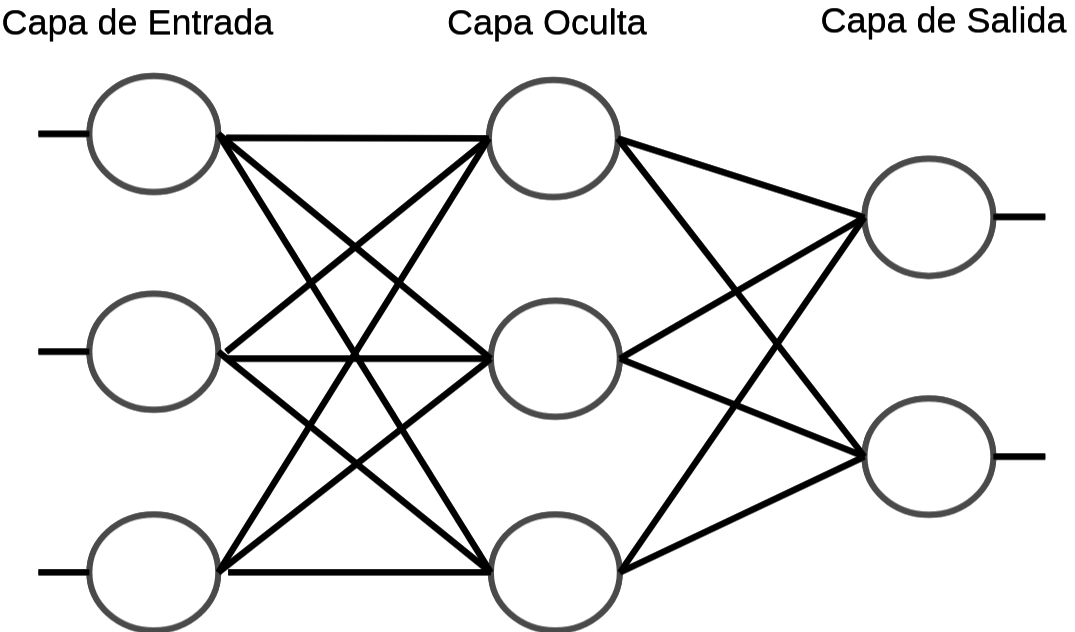
\includegraphics[width=0.5\textwidth]{MarcoTeorico/imgs/MLP.png}
    \caption{Representación básica de red neuronal multicapa.}
    \label{fig:mlp}
\end{figure}

Los MLP también se conocen como aproximadores universales, ya que pueden encontrar la relación entre los valores de entrada y los objetivos, utilizando una cantidad suficiente de neuronas en la capa oculta, alterando los pesos o utilizando datos de entrenamiento adicionales para aproximar la función dada hasta cualquier nivel de precisión. A menudo, con el grado de libertad dado a un MLP, puede superar a la red MLP básica, introduciendo más capas ocultas, con menos neuronas en cada una de las capas ocultas y pesos óptimos. Esto ayuda en el proceso de generalización general del modelo (\cite{goyal2018Deep}).

\subsection{Propagación hacia atrás(Backpropagation)}

En las redes neuronales es complicado ajustar sus pesos de entrenamiento por la gran cantidad de conexiones y sus múltiples niveles. Para lograr esta tarea, se utiliza el algoritmo backpropagation, creado por \citeauthor{rumelhart1986Parallel} en \citeyear{rumelhart1986Parallel}.

En el algoritmo Backpropagation calculamos qué tan rápido cambia el error a medida que cambiamos una capa oculta. A partir de ahí, podemos averiguar qué tan rápido cambia el error cuando cambiamos el peso de una conexión individual. Básicamente, intentamos encontrar el camino de descenso más empinado. Comenzamos calculando las derivadas del error con respecto a un solo ejemplo de entrenamiento. Una vez que tenemos las derivadas de error para una capa de unidades ocultas, las usaremos para calcular las derivadas de error para las unidades de la capa siguiente. Y una vez que encontramos las derivadas del error para las actividades de las unidades ocultas, es bastante fácil obtener las derivadas del error para los pesos que conducen a una unidad oculta (\cite{buduma2017Fundamentals}).

En resumen, el algoritmo backpropagation consiste en dos pasos como muestra la figura:

\begin{itemize}
\item Propagación hacia adelante: Se calculan los pesos de cada una de las neuronas, desde la capa de entrada hasta la capa de salida.

\item Propagación hacia atrás: Se calcula el error y se actualizan los pesos, desde la capa de salida hasta la capa de entrada.
\end{itemize}

\begin{figure}[H]
    \centering
    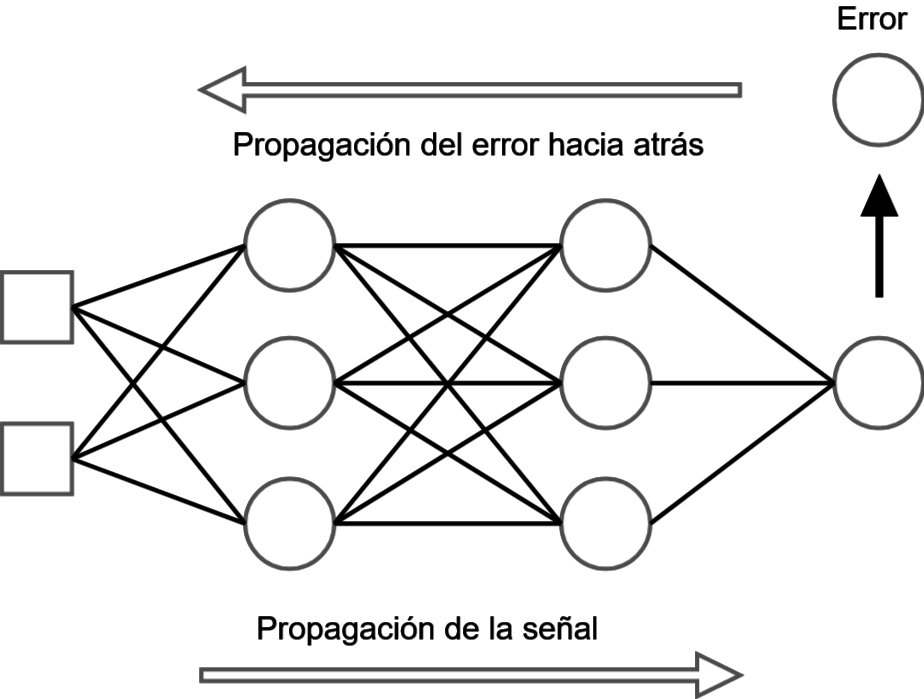
\includegraphics[width=0.8\textwidth]{MarcoTeorico/imgs/Backpropagation.png}
    \caption{Propagación hacia adelante y propagación hacia atrás.}
    \label{fig:backpropagation}
\end{figure}

\subsection{Descenso del Gradiente }

El método del descenso del gradiente es un algoritmo iterativo que minimiza una función de pérdida actualizando posteriormente los parámetros de la función.

\begin{figure}[H]
    \centering
    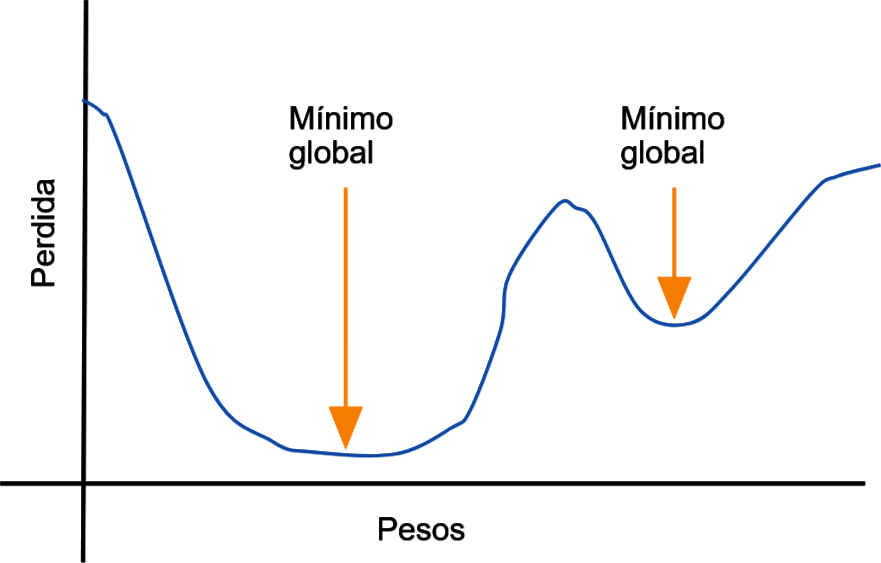
\includegraphics[width=0.8\textwidth]{MarcoTeorico/imgs/DescensoGradiente.png}
    \caption{Mínimo local y global.}
    \label{fig:descensoGradiente}
\end{figure}

La Figura \ref{fig:descensoGradiente} muestra cómo podemos tener múltiples picos y valles (Máximos y mínimos) para nuestros valores de perdida. El valor ideal que nos gustaría obtener es nuestro mínimo global, asegurando que nuestros parámetros tomen los valores más óptimos posibles.

El problema es que no tenemos una vista general en la que podamos encontrar de manera sencilla el mínimo global ya que en realidad nos colocaríamos en un lugar aleatorio sin saber dónde está el mínimo global y tendríamos que avanzar hacia una perdida mínima sin subir accidentalmente a la cima de un máximo local.

\subsection{Tasa de aprendizaje}

La tasa de aprendizaje es uno de los hiperparámetros más importantes. Tiene un fuerte impacto tanto en la estabilidad como en la eficiencia de los tiempos de entrenamiento y no hay una forma fija de encontrar la más adecuada. La tasa de aprendizaje es la magnitud del ajuste de pesos durante el entrenamiento de la red con el fin de minimizar el error (\cite{valenzuela2020Sistema}).

La imagen muestra que si la tasa es demasiado grande, nuestro entrenamiento es inestable. Si nuestra tasa de aprendizaje es demasiado pequeña, el entrenamiento puede tomar más tiempo para llegar a un entrenamiento adecuado.

\begin{figure}[H]
    \centering
    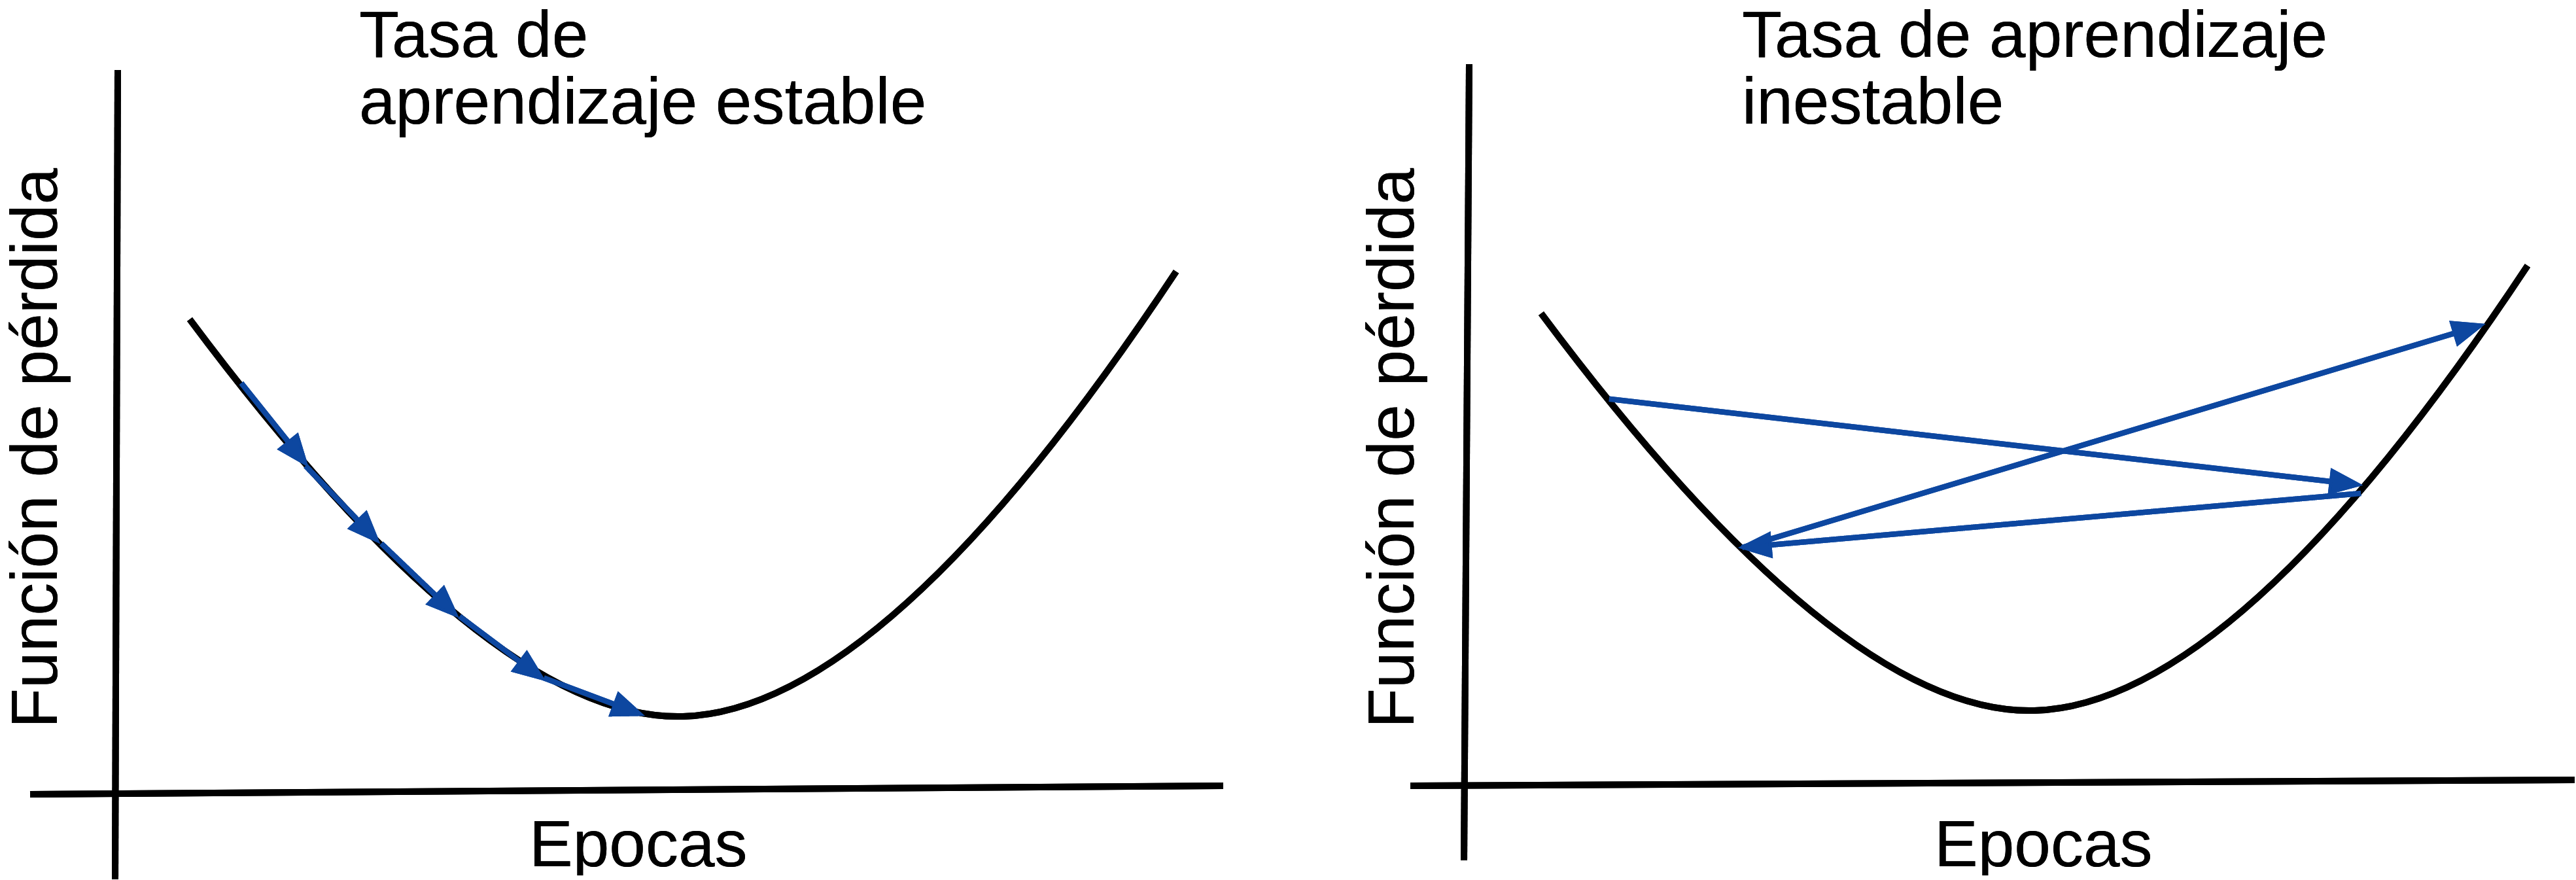
\includegraphics[width=0.8\textwidth]{MarcoTeorico/imgs/LearningRate.png}
    \caption{Tasa de aprendizaje.}
    \label{fig:learningRate}
\end{figure}

Preferiblemente, nuestra pérdida de entrenamiento y validación casi se imitan entre sí, con solo una pequeña brecha entre la pérdida de entrenamiento y la pérdida de validación, lo que indica un pequeño sobreajuste. Siempre que la brecha no aumente drásticamente, sabemos que existe un nivel aceptable de sobreajuste. Por otro lado, si no logramos mantener esta brecha y las pérdidas de entrenamiento y validación se separan drásticamente, entonces sabemos que corremos el riesgo de sobreajuste. Una vez que la pérdida de validación comienza a aumentar, sabemos que estamos muy sobreajustados (\cite{rosebrock2017deep}).


\subsection{Funciones de activación}

Las funciones de activación son una función de escalar a escalar, que produce la activación de la neurona. Usamos funciones de activación para propagar la salida de los nodos de una capa hacia la siguiente capa. Usamos funciones de activación para neuronas ocultas en una red neuronal para introducir la no linealidad del modelado de la red (\cite{patterson2017deep}).

